\scanpage{75}
diagramme qui est déterminé, à isom. unique près, en se donnant un ordre total sur $I$, \inserted{(défini} mod \deleted{\unsure{interversion}} \inserted{transposition} des deux premiers él, et des deux derniers). Pour montrer que deux ordres totaux sur $I$ définissent \deleted{une} des pts de $M^\infty_{0,\nu}$ qui appartiennent à une $=$ composante connexe, il \inserted{suffit de} montrer que deux ordres totaux déduits l'un de l'autre par transposition des deux élts consécutifs \inserted{$c_i,c_{i+1}$} sont dans la $=$ composante connexe. Or on le voit en notant qu'on a deux morphismes de spécialisation \deleted{de} \inserted{dans}
\figure{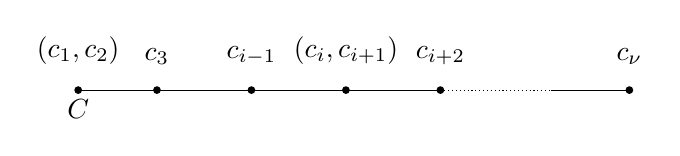
\begin{tikzpicture}[x=1cm,y=1cm]
\draw (0,0)--(1,0)--(2.2,0)--(3.4,0)--(4.6,0);
\draw[densely dotted] (4.6,0)--(6,0);\draw (6,0)--(7,0);
\foreach \x in {0,1,2.2,3.4,4.6,7}{\fill (\x,0) circle (1.4pt);}
\node[above] at (0,.2) {$(c_1,c_2)$};\node[below] at (0,0) {$C$};
\node[above] at (1,.2) {$c_3$};\node[above] at (2.2,.2) {$c_{i-1}$};
\node[above] at (3.4,.2) {$(c_i,c_{i+1})$};\node[above] at (4.6,.2) {$c_{i+2}$};
\node[above] at (7,.2) {$c_\nu$};
\end{tikzpicture}}
provient de
\figure{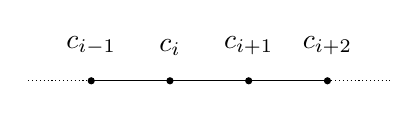
\begin{tikzpicture}[x=1cm,y=1cm]
\draw[densely dotted] (-.8,0)--(0,0) (3,0)--(3.8,0);\draw (0,0)--(1,0)--(2,0)--(3,0);
\foreach \x in {0,1,2,3}{\fill (\x,0) circle (1.3pt);}
\node[above] at (0,.2) {$c_{i-1}$};\node[above] at (1,.2) {$c_i$};
\node[above] at (2,.2) {$c_{i+1}$};\node[above] at (3,.2) {$c_{i+2}$};
\end{tikzpicture}}
et de
\figure{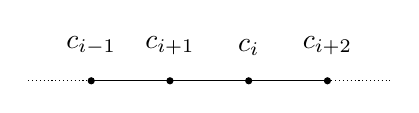
\begin{tikzpicture}[x=1cm,y=1cm]
\draw[densely dotted] (-.8,0)--(0,0) (3,0)--(3.8,0);\draw (0,0)--(1,0)--(2,0)--(3,0);
\foreach \x in {0,1,2,3}{\fill (\x,0) circle (1.3pt);}
\node[above] at (0,.2) {$c_{i-1}$};\node[above] at (1,.2) {$c_{i+1}$};
\node[above] at (2,.2) {$c_i$};\node[above] at (3,.2) {$c_{i+2}$};
\end{tikzpicture}}
en contractant la \deleted{\unsure{seg}} \inserted{arête} qui joint $c_i$ et $c_{i+1}$, OK.
\margin{74}
